\documentclass[11pt]{beamer}
\usepackage[MeX]{polski}
\usepackage[utf8]{inputenc}
\usepackage{amsmath}
\usepackage{amsfonts}
\usepackage{amssymb}
\usepackage{graphicx}
\usetheme{CambridgeUS}
\usecolortheme{beaver}
\usepackage{textpos}
\begin{document}
	\author[S.Z, P.S.]{Sebastian Zając, Piotr Sułkowski}
	\title{Topologiczna charakterystyka RNA i białek}
	\institute{WMP.SNŚ UKSW\\ WF UW}
	\date{19 marca 2017}
	%\subject{}
	%\setbeamercovered{transparent}
	%\setbeamertemplate{navigation symbols}{}
	\begin{frame}	
			\maketitle
	\end{frame}
		
	\begin{frame}	
	\frametitle{Fizyka}
	\begin{center}
		
\includegraphics[scale=0.15]{feydiag}
	\end{center}
		\end{frame}
		\begin{frame}	
		\frametitle{Topologia}
		\begin{center}
			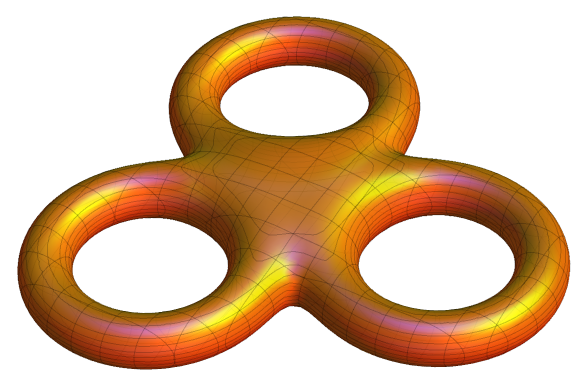
\includegraphics[scale=0.5]{genus}
		\end{center}
	\end{frame}
\frame{
	\frametitle{RNA}
	\begin{center}
		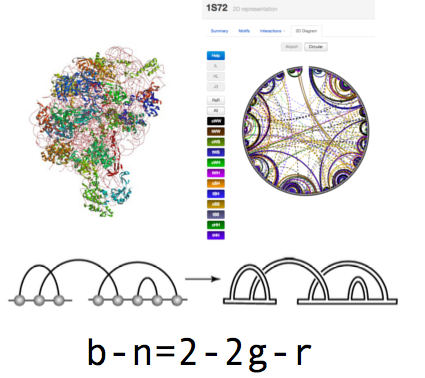
\includegraphics[scale=0.5]{rna.png}
	\end{center}
}
\frame{
\frametitle{Baza PDB}
\begin{center}
	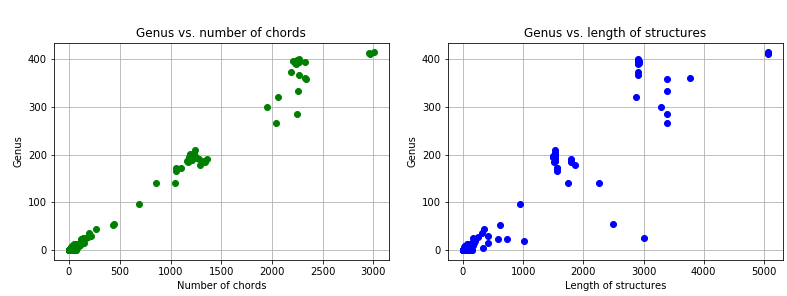
\includegraphics[scale=0.44]{rys1.png}
\end{center}
}
\frame{
\frametitle{1S72}
\begin{center}
	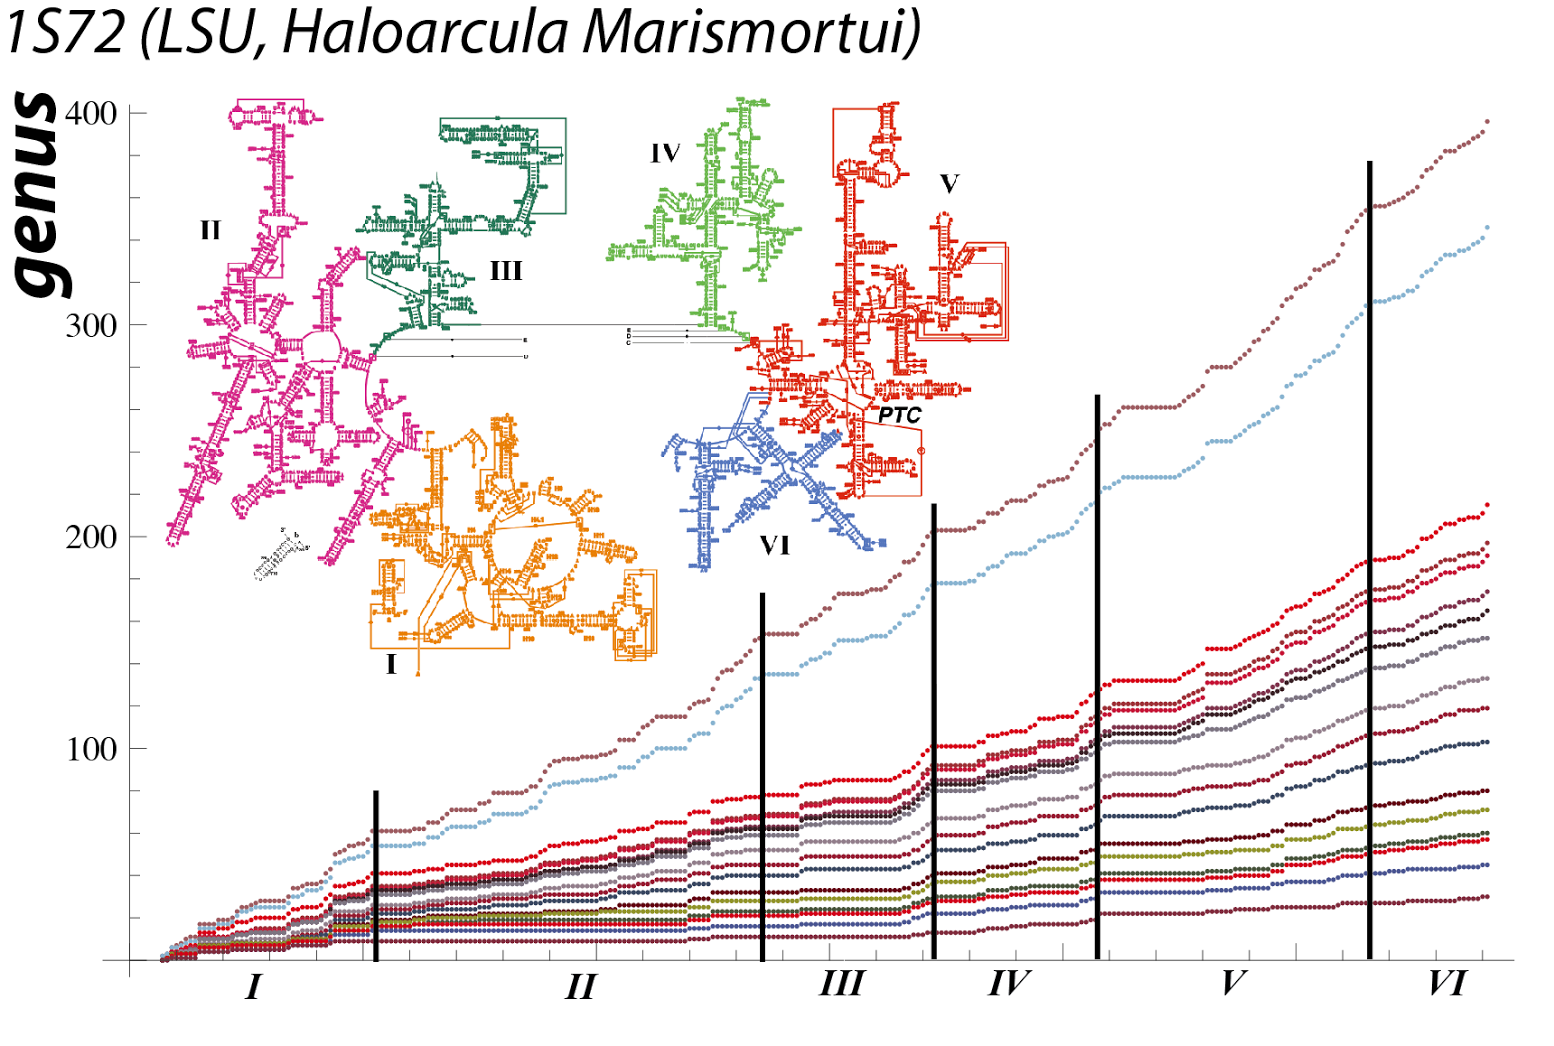
\includegraphics[scale=0.2]{ribogenus2.png}
\end{center}
}
\frame{
\frametitle{Białka}
\begin{center}
	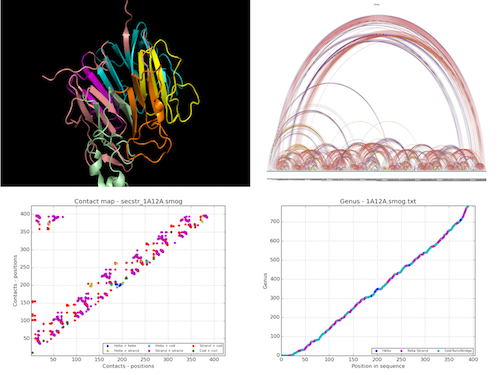
\includegraphics[scale=0.5]{protein.png}
\end{center}
}
\end{document}